Things get more interesting in perspective of expressing $\E[\norm{\bar{x}_{t+1} - x_*}^2]$ through $\E[\norm{\bar{x}_{t} - x_*}^2]$ instead of solving recurrent relation and analyzing $\E[\norm{\bar{x}_T - x_*}^2]$. 

We'll go deeper into the highly convex case because it's more intuitive.

As can be observed from~\ref{lem:main}:
\begin{align}
     \E \norm{\bar{x}_{t+1}-x_*}^2
    &\leq
    (1 - \gamma \mu) \E \norm{\bar{x}_t - x_*}^2 
    + \frac{\gamma^2 \sigma^2}{M}
    + 10 \varepsilon \gamma L (H-1) \gamma^2 \sigma^2 \label{eq:recurrent}
\end{align}

Considering $\varepsilon$ as a function of $x$, we can say that for the functions with Lipschitz Hessian we know that the decay rate of $\varepsilon$ is fast. Following graphs illustrate decay rate of $\varepsilon$ for some functions:

\begin{figure}[H] \label{graph:eps_graphs}
\centering
\begin{subfigure}{0.3\textwidth}
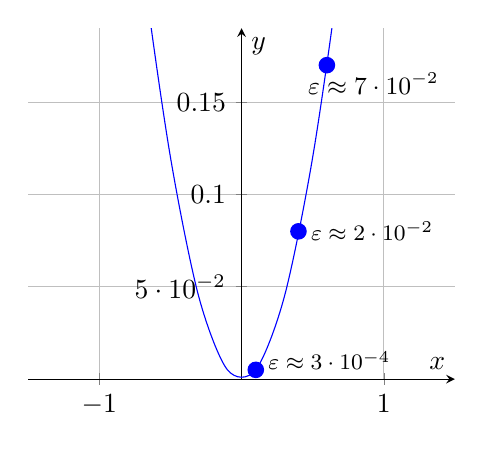
\begin{tikzpicture}
\begin{axis}[
    width=7cm,
    xlabel={$x$},
    ylabel={$y$},
    xmin=-1.5, xmax=1.5,
    ymin=0, ymax=0.19, % Adjust y-axis limits
    axis lines=center,
    grid=both,
    domain=-10:10,
    samples=100,
    % restrict y to domain=-2.5:2.5 % Restrict y-axis domain
]

\addplot[blue, smooth] {ln(cosh(x))};

\coordinate (A1) at (axis cs:0.6,0.17);
\coordinate (B1) at (axis cs:0.4,0.16);

\fill[blue, thick] (A1) circle (3pt);
\node[right] at (B1) {\small $\bm{\varepsilon \approx 7 \cdot 10^{-2}}$};

%\draw[dashed] (A1) -- (B1);
 %----------------------------------------%
\coordinate (A2) at (axis cs:0.4,0.08);
\coordinate (B2) at (axis cs:0.42,0.08);

\fill[blue, thick] (A2) circle (3pt);
\node[right] at (B2) {\footnotesize $\bm{\varepsilon \approx 2 \cdot 10^{-2}}$};

%\draw[dashed] (A2) -- (B2);
 %----------------------------------------%
% \coordinate (A3) at (axis cs:0.2,0.02);
% \coordinate (B3) at (axis cs:0.35,0.03);

% \fill[blue, thick] (A3) circle (3pt);
% \node[right] at (B3) {\footnotesize $\bm{\varepsilon \approx 2 \cdot 10^{-3}}$};

% \draw[dashed] (A3) -- (B3);
%----------------------------------------%
\coordinate (A4) at (axis cs:0.1,0.005);
\coordinate (B4) at (axis cs:0.12,0.01);

\fill[blue, thick] (A4) circle (3pt);
\node[right] at (B4) {\footnotesize $\bm{\varepsilon \approx 3 \cdot 10^{-4}}$};

%\draw[dashed] (A4) -- (B4);

\end{axis}
\end{tikzpicture}
\caption{LogCoshLoss: $y = \ln(\cosh(x))$ }
\end{subfigure}
\hfill
\begin{subfigure}{0.3\textwidth}
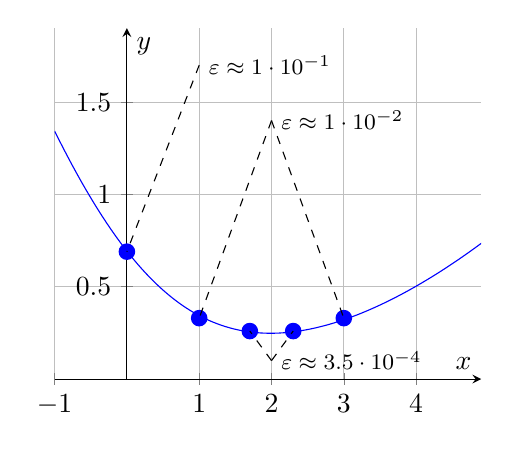
\begin{tikzpicture}
\begin{axis}[
    width=7cm,
    xlabel={$x$},
    ylabel={$y$},
    xmin=-1, xmax=4.9,
    ymin=-0, ymax=1.9,
    axis lines=center,
    grid=both,
    samples=100,
]
\addplot[blue, domain=-1:5] {-ln(1/(1 + exp(-x))) + x^2/33};

\coordinate (A1) at (axis cs:1, 0.33);
\coordinate (B1) at (axis cs:2, 1.4);
\coordinate (C1) at (axis cs:3,0.33);

\fill[blue, thick] (A1) circle (3pt);
\fill[blue, thick] (C1) circle (3pt);
\node[right] at (B1) {\footnotesize $\bm{\varepsilon \approx 1 \cdot 10^{-2}}$};

\draw[dashed] (B1) -- (A1);
\draw[dashed] (B1) -- (C1);
 %----------------------------------------%
\coordinate (A2) at (axis cs:1.7, 0.26);
\coordinate (B2) at (axis cs:2, 0.1);
\coordinate (C2) at (axis cs:2.3,  0.26);

\fill[blue, thick] (A2) circle (3pt);
\fill[blue, thick] (C2) circle (3pt);
\node[right] at (B2) {\footnotesize $ \bm{\varepsilon \approx 3.5 \cdot 10^{-4}}$};

\draw[dashed] (B2) -- (A2);
\draw[dashed] (B2) -- (C2);
 %----------------------------------------%
 \coordinate (A2) at (axis cs:0, 0.69);
\coordinate (B2) at (axis cs:1, 1.7);

\fill[blue, thick] (A2) circle (3pt);
\node[right] at (B2) {\footnotesize $\bm{\varepsilon \approx 1 \cdot 10^{-1}}$};

\draw[dashed] (B2) -- (A2);
 %----------------------------------------%
\end{axis}
\end{tikzpicture}
\caption{LogLoss with $l_2$ reg.  ~\eqref{eq:logloss}}
\end{subfigure}
\hfill
\begin{subfigure}{0.3\textwidth}
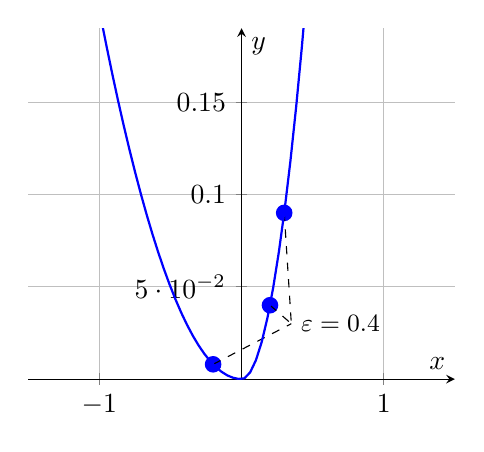
\begin{tikzpicture}[
  declare function={
    func(\x)= (\x < 0) * (x*x/5)   +
              (\x >= 0) * (x*x)
   ;
  }
]
\begin{axis}[
    width=7cm,
    xlabel={$x$},
    ylabel={$y$},
    xmin=-1.5, xmax=1.5,
    ymin=0, ymax=0.19, % Adjust y-axis limits
    axis lines=center,
    grid=both,
    domain=-2:2,
    samples=100,
    % restrict y to domain=-2.5:2.5 % Restrict y-axis domain
]

\coordinate (A1) at (axis cs:-0.2,0.008);
\coordinate (A2) at (axis cs:0.2,0.04);
\coordinate (A3) at (axis cs:0.3,0.09);

\coordinate (B1) at (axis cs:0.35,0.03);

\fill[blue, thick] (A1) circle (3pt);
\fill[blue, thick] (A2) circle (3pt);
\fill[blue, thick] (A3) circle (3pt);


\node[right] at (B1) {\small $\bm{\varepsilon = 0.4}$};

\draw[dashed] (A1) -- (B1);
\draw[dashed] (A2) -- (B1);
\draw[dashed] (A3) -- (B1);

\addplot [blue,thick] {func(x)};
\end{axis}
\end{tikzpicture}
\caption{Lower-bound function $\mathcal{F} $ ~\eqref{eq:piecewise}}
\end{subfigure}


\caption{Decay of $\varepsilon$ when getting closer to minima}
\end{figure}
\\

In point (b) by LogLoss we consider 
\begin{equation} \label{eq:logloss}
    y = -\ln\left(\frac{1}{1 + e^{-x}} \right) + 0.03 {x^2}
\end{equation}

And in point (c) we analyze well-known function that yields lower bound estimates for Local SGD \citep{LowerBound}.
\begin{equation} \label{eq:piecewise}
    \mathcal{F}(x) = \begin{cases} 
      x^2 / 5 & \text{if } x < 0 \\
      x^2 & \text{if } x \geq 0 \\
   \end{cases}
\end{equation}

Here we can notice that for functions (a) and (b) $\varepsilon$ decreases rapidly because they satisfy Lipschitz Hessian assumption, and for function (c) it remains constant. This may be considered as some additional insight into why 
$\mathcal{F}$ yields lower bound for Local SGD.

From this example we can observe that equation~\ref{eq:recurrent} provides valuable insights into convergence rate for different types of functions. However, abandoning the assumption of a Lipschitz Hessian means that we cannot estimate the decay rate of epsilon. Therefore conducting a meaningful asymptotic analysis while maintaining generality seems impossible.

Thus our aim is to present our findings within a broader scope, elucidating the physical interpretation of the convergence rate.
